\section{The user interface}
\label{sec:hooke:ui}

\Hooke commands are written with abstract argument definitions (using
the cleverly named \imint{python}|Argument| class).  This makes it
easier to add new user interfaces (UIs), because the user interface is
fundamentally about selecting commands and arguments to pass to them.
In my work on \Hooke, I borrowed from the graphical user interface
(GUI) version from Concordia with the original
partially-command-line-version from Bologna to produce two independent
interfaces: a command line interface (CLI) and the GUI.  You can do
exactly the same things in either interface; choosing whichever is
most convenient for the task at hand
(\cref{fig:hooke:cli,fig:hooke:gui}).  I usually use the CLI for
scripting and routine tasks and reproducible analysis, but fire up the
GUI when I'm exploring new data.

\begin{figure}
  \begin{center}
\begin{minted}{console}
$ hk.py
Hooke version 1.0.0.alpha (Ninken)
...
----
hooke> new_playlist --output_playlist mylist
<FilePlaylist mylist>
Success

hooke> glob_curves_to_playlist *.jpk
<Curve 2009.04.23-15.15.47.jpk>
<Curve 2009.04.23-15.21.39.jpk>
Success

hooke> curve_info
name: 2009.04.23-15.15.47.jpk
path: /.../hooke/test/data/vclamp_jpk/2009.04.23-15.15.47.jpk
driver: <hooke.driver.jpk.JPKDriver object at 0x28f9710>
note: None
command stack: []
blocks: 2
block names: ['approach', 'retract']
block sizes: [(4096, 6), (4096, 4)]
Success
\end{minted}
    \caption{Creating a playlist with two JPK files in the Hooke
      command line interface.\label{fig:hooke:cli}}
  \end{center}
\end{figure}

\begin{figure}
  \begin{center}
    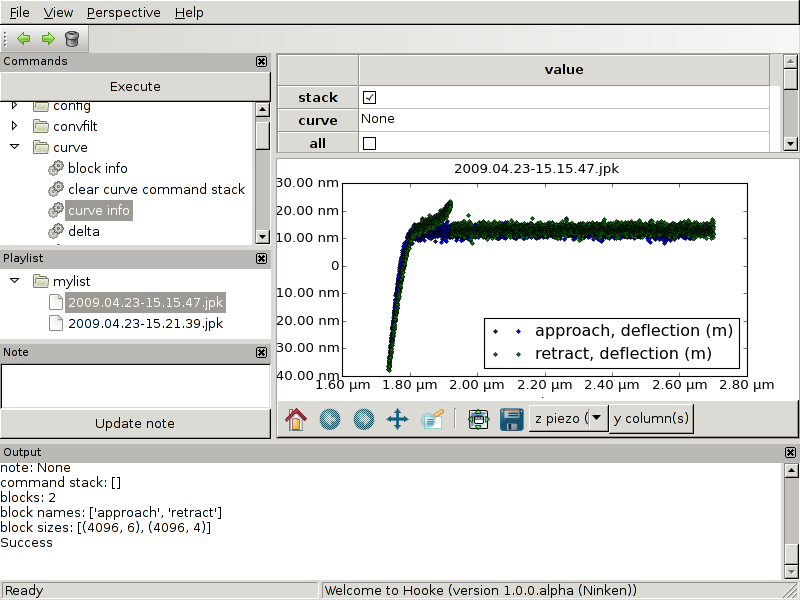
\includegraphics[width=\textwidth]{figures/binary/hooke-gui}
    \caption{Creating a playlist with two JPK files in the graphical
      Hooke interface.  You can see the output of the last \gui{curve
        info} call, which matches the output from the command line
      version (\cref{fig:hooke:cli}).  This screenshot is a bit
      cramped (to fit on a printed page), but the
      \href{http://www.wxwidgets.org}{wxWidgets} GUI toolkit provides
      automatic support for interactively rearranging and resizing
      panels.  The tree of commands is in the upper left corner.
      After you select a command, the table of argument in the upper
      right corner is populated with default values, which you can
      adjust as you see fit.  The \gui{Playlist} panel provides an
      easier interface for navigating to different playlists and
      curves than the using \gui{jump to playlist} and \gui{jump to
        curve} commands.\label{fig:hooke:gui}}
  \end{center}
\end{figure}
